The source code of the module described in this document can be found at the following GitHub repository:
\url{https://github.com/andreafontana99/MBDyn-MFtire}
\section{Introduction}
This document provides an overview of the MFtire module for MBDyn, which implements a single contact point Pacejka tire model intended for full-vehicle handling simulations in a multibody environment.
This is the second iteration of the module (effectively v0.2), where a complete refactoring of the slip calculation has allowed to remove some simplifying assumptions, improving the slip accuracy under high camber rates.

Some aspects to keep in mind:
\begin{itemize}
    \item It's still a work in progress
    \item The formulation is intentionally simple for three main reasons:
        \begin{itemize}
            \item Low computational cost is mandatory for real-time simulations
            \item The number of required parameters (e.g. tire data) must be low
            \item The development of the jacobian matrix, necessary to guarantee stability and fast convergence, is straightforward but quite involved. As the number of calculations in the residual grows, the Jacobian components may become cumbersome to develop, debug, and maintain (as the process is still not automated).
    \end{itemize}
    \item Most of the effort has been focused on the proper formulation of tire input quantities—such as slip angle, slip ratio, camber angle, and loaded radius—while less emphasis has been placed on the definition of forces and moments. This makes the module a solid starting point for users interested in implementing their own force and moment formulas.
\end{itemize}

Section~\ref{sec:residual} calculations are based on \cite{pacejka2012tireChap5}. Note that both the sign conventions for the reference frame vectors and the notation are substantially different.

\section{Model capabilities}
The module calculates the forces and moments and applies them to the connected rim node. For now, pure longitudinal and lateral forces are directly computed as function of slips and vertical load while tire moments are still to be implemented. Combined effects and camber dependency of the forces and rolling radius are neglected as well as relaxation effects.
The vertical load is obtained by computing the difference between the instant and the undeformed loaded radius, which is then multiplied by a constant stiffness.

\section{TODO}
\begin{itemize}
    \item Self-aligning moment
    \item Combined effects
    \item Non-linear vertical stiffness and damping
    \item Relaxation effects (hopefully this removes the need for low speed handling)
    \item Rolling resistance
    \item Ground mesh
    \item Handling of wheel detachment
    \item NetCDF output
\end{itemize}

\section{I/O and module interface}

% \begin{lstlisting}[escapeinside={(*@}{@*)}]
% (*@\textcolor{red}{user defined}@*): <tire_label>, MFtire,
%     # wheel structural node label
%     <hub_node_label>,
%     <rim_node_label>,
%     # wheel axle direction (e.g. 0., 1., 0.)
%     <Vec3_axle>,
%     # unloaded radius
%     <Ru>,
%     # effective rolling radius
%     <Re>,
%     # tire vertical stiffness
%     <kt>,
%     # longitudinal pacejka coefficients
%     <Dx>, <Cx>, <Bx>, <Ex>,
%     # lateral pacejka coefficients
%     <Dy>, <Cy>, <By>, <Ey>,
%     # reference vx, damping coeff
%     low speed, <vx_low>, <vx_dmp>;
% \end{lstlisting}

\section{Notation}
\subsection*{Identity matrix}
\begin{equation}
    \mathbf{I}_{3\times3} = \begin{bmatrix}
                                1 & 0 & 0 \\
                                0 & 1 & 0 \\
                                0 & 0 & 1
                            \end{bmatrix}
\end{equation}
\subsection*{Cross product}
\begin{equation}
    \mathbf{a} \times \mathbf{b} = \det\begin{bmatrix}
                                \mathbf{e}_1 & \mathbf{e}_2 & \mathbf{e}_3 \\
                                a_1 & a_2 & a_3 \\
                                b_1 & b_2 & b_3
                            \end{bmatrix} = a_i b_i \epsilon_{ijk} \mathbf{e}_k
\end{equation}
where $\epsilon_{ijk}$ is the permutation symbol (Levi-Civita) and $\mathbf{e}_i$ for $i = 1,2,3$ are the cartesian base vectors.
\subsection*{Skew-symmetric matrix}
A matrix resulting from the application of the cross-product operator to a three-dimensional
vector
\begin{equation}
    \mathbf{v} \times = \begin{bmatrix}
                                0 & -v_z & v_y \\
                                v_z & 0 & -v_x \\
                                -v_y & v_x & 0
                            \end{bmatrix}
\end{equation}
\subsection*{Dyadic product}
\begin{equation}
    \mathbf{v} \otimes \mathbf{v} = \mathbf{v}\mathbf{v}^T
\end{equation}
\section{Residual assembly}
\label{sec:residual}
\section{Ground}
The ground surface is defined by mapping to each $(x,y)$ coordinate a position vector and a unit normal vector, denoted as $\mathbf{q}$ and $\mathbf{n}$, respectively. To simplify the derivation, a flat and constant plane is assumed; therefore, $\mathbf{q}$ and $\mathbf{n}$ are constant vectors given by:
\begin{equation}
\label{eq:assumptions}
\mathbf{q} = \mathbf{0}\hspace{1cm}\mathbf{n} = \begin{bmatrix}
0 & 0 & 1
\end{bmatrix}^T
\end{equation}

\section{Hub carrier and rim kinematics}
Two nodes are required to fully describe the contact point kinematics: the wheel hub node and the rim node. The wheel hub and the rim must be constrained to rotate around the wheel spindle axis, denoted by $\tilde{s}$, which is constant in the local reference frame of the wheel hub. Both nodes must be coincident with the wheel centre.
The position, velocity, and orientation matrix of the wheel hub node are denoted by $\mathbf{w}_H$, $\dot{\mathbf{w}}_H$, and $\mathbf{R}_H$, respectively, while the angular velocity of the rim is $\boldsymbol{\omega}_R$.

\section{Reference frame}
The following vectors, following the ISO sign convention, define the directions along which the forces act and enable the computation of the contact point position and velocity.
The wheel spin axis representation in the global reference frame is:
\begin{equation}
    \mathbf{s} = \mathbf{R}_H \tilde{\mathbf{s}}
\end{equation}
$\mathbf{s}$ is a unit length vector as the input local spin axis is normalized.
The local forward ($\mathbf{l}$) and transverse ($\mathbf{t}$) directions can be obtained as follows:
\begin{equation}
    \begin{split}
        \mathbf{l} &= \frac{\mathbf{s} \times \mathbf{n}}{||\mathbf{s} \times \mathbf{n}||}\\
        \mathbf{t} &= \mathbf{n} \times \mathbf{l}
    \end{split}
\end{equation}
The radial direction $\mathbf{r}$ is perpendicular both to $\mathbf{s}$ and $\mathbf{l}$:
\begin{equation}
    \mathbf{r} = \mathbf{l} \times \mathbf{s}
\end{equation}
The time derivatives of the unit vectors are:
\begin{equation}
    \begin{split}
        \dot{\mathbf{s}} &= \boldsymbol{\omega}_R \times \mathbf{s} \\
        \dot{\mathbf{l}} &= \frac{\mathbf{I}_{3\times3} - \mathbf{l} \otimes \mathbf{l}}{||\mathbf{s} \times \mathbf{n}||}\left(\dot{\mathbf{s}} \times \mathbf{n}\right) \\
        \dot{\mathbf{t}} &= \mathbf{n} \times \dot{\mathbf{l}} \\
        \dot{\mathbf{r}} &= \dot{\mathbf{l}} \times \mathbf{s} + \mathbf{l} \times \dot{\mathbf{s}}
    \end{split}
\end{equation}

These expressions rely on the assumption that $\dot{\mathbf{n}} = \mathbf{0}$, as the road plane is constant, and must be modified accordingly in case a general rigid/deformable surface is considered.

Note that the lateral direction points to the left and the radial direction is positive upwards.

\section{Loaded radius}
To obtain the magnitude of the loaded radius, $\rho$, let's first define the position of the contact point:
\begin{equation}
    \mathbf{c} = \mathbf{w}_H + \rho\mathbf{r}
\end{equation}
The contact point and the road point must lie on the same plane perpendicular to $\mathbf{n}$, which translates in the following equation:
\begin{equation}
    \mathbf{c} \cdot \mathbf{n} = \mathbf{q} \cdot \mathbf{n}
\end{equation}
As $\mathbf{q} = \mathbf{0}$, this expression can be simplified to:
\begin{equation}
    \begin{split}
        \mathbf{0} &= \mathbf{c} \cdot \mathbf{n} \\
        \mathbf{0} &= \left(\mathbf{w}_H + \rho\mathbf{r}\right) \cdot \mathbf{n}
    \end{split}
\end{equation}
Therefore,
\begin{equation}
    \rho = -\frac{\mathbf{w}_H \cdot \mathbf{n}}{\mathbf{r} \cdot \mathbf{n}}
\end{equation}
The derivative of the loaded radius is the following:
\begin{equation}
    \dot{\rho} = -\frac{\left(\dot{\mathbf{w}}_H  + \rho \dot{\mathbf{r}}\right)\cdot \mathbf{n}}{\mathbf{r} \cdot \mathbf{n}}
\end{equation}

Note that as $\rho\mathbf{r}$ is a vector from the wheel center to the contact point and $\mathbf{r}$ points up, $\rho$ is always negative in normal operating conditions (e.g. unless you are driving upside down).

\section{Slip Quantities}

The velocity of the contact point $\mathbf{c}$ is:
\begin{equation}
    \begin{split}
        \mathbf{v}_{C} &= \dot{\mathbf{w}}_H + \frac{d\left(\rho\mathbf{r}\right)}{dt} \\
        &= \dot{\mathbf{w}}_H + \dot{\rho}\mathbf{r} + \rho\mathbf{r}
    \end{split}
\end{equation}
The speed of propagation of the point $\mathbf{c}^*$ is:
\begin{equation}
    \begin{split}
        \mathbf{v}_{C}^* &= \dot{\mathbf{w}}_H - \frac{r_e}{\rho}\frac{d\left(\rho\mathbf{r}\right)}{dt} \\
        &= \dot{\mathbf{w}}_H - \frac{r_e}{\rho}\dot{\rho}\mathbf{r} - r_e\mathbf{r}
    \end{split}
\end{equation}
Note that scaling the second term by $\frac{r_e}{\rho}$ also requires a change in sign due to the fact that $\rho$ is negative.
The velocity of point $\mathbf{s}$ that is fixed to the wheel body reads:
\begin{equation}
    \begin{split}
        \mathbf{v}_{S} &= \dot{\mathbf{w}}_H - \frac{r_e}{\rho} \boldsymbol{\omega}_R \times \left(\rho\mathbf{r}\right) \\
        &= \dot{\mathbf{w}}_H - r_e \boldsymbol{\omega}_R \times \mathbf{r}
    \end{split}
\end{equation}
The following velocity components allow for an easier definition of the slip quantities:
\begin{equation}
    \begin{split}
        v_x &= \mathbf{v}_{C}^* \cdot \mathbf{l} \\
        v_y &= \mathbf{v}_{C} \cdot \mathbf{t} \\
        v_s &= \mathbf{v}_{S} \cdot \mathbf{l}
    \end{split}
\end{equation}
$r_e$ is the (constant, for now) effective rolling radius.
Longitudinal and lateral theoretical slips require particular care to avoid numerical instability as longitudinal speed approaches zero. As frequently found in vehicle dynamics literature, ad hoc definitions of slip quantities are adopted below a given speed threshold ($v_{x, \text{LOW}}$), denoted as $\alpha_L$ and $\kappa_L$, to avoid division by zero. Above that threshold, the standard definitions are applied, $\alpha_H$ and $\kappa_H$.
\begin{equation}
    \begin{split}
        \alpha_H &= \arctan\left(\frac{v_y}{v_x}\right)\\
        \kappa_H &= -\frac{v_s}{v_x}
    \end{split}
\end{equation}
\begin{equation}
    \begin{split}
        \alpha_L &= v_y\\
        \kappa_L &= -v_s
    \end{split}
\end{equation}
Where the $\arctan(x)$ function is implemented as $atan2$.

The two functions
\begin{equation}
    \kappa =
    \begin{cases}
        \kappa_L & \text{if } |v_x| \leq v_{x,\text{LOW}}, \\
        \kappa_H & \text{if } |v_x| > v_{x,\text{LOW}}, \\
    \end{cases}
\end{equation}
\begin{equation}
    \alpha =
    \begin{cases}
        \alpha_L & \text{if } |v_x| \leq v_{x,\text{LOW}}, \\
        \alpha_H & \text{if } |v_x| > v_{x,\text{LOW}}, \\
    \end{cases}
\end{equation}
are not continuous at $v_x = v_{x,\text{LOW}}$. To smoothly transition between the two definitions, a function $\chi$ is introduced. This also allows to obtain a single continuous function which can be differentiated and easily included in the model Jacobian matrix. The parameter $v_{x, \text{DMP}}$ allows to tune how quickly the transition between low speed and high speed state happens.
\begin{equation}
    \chi = \frac{1}{2}\left[\tanh\left(\frac{|v_x| - v_{x, \text{LOW}}}{v_{x, \text{DMP}}}\right) + 1\right]
\end{equation}
The expression for the derivative of $\chi$, needed in the Jacobian matrix, is reported in \ref{ss:derivatives}
\begin{figure}
    \centering
    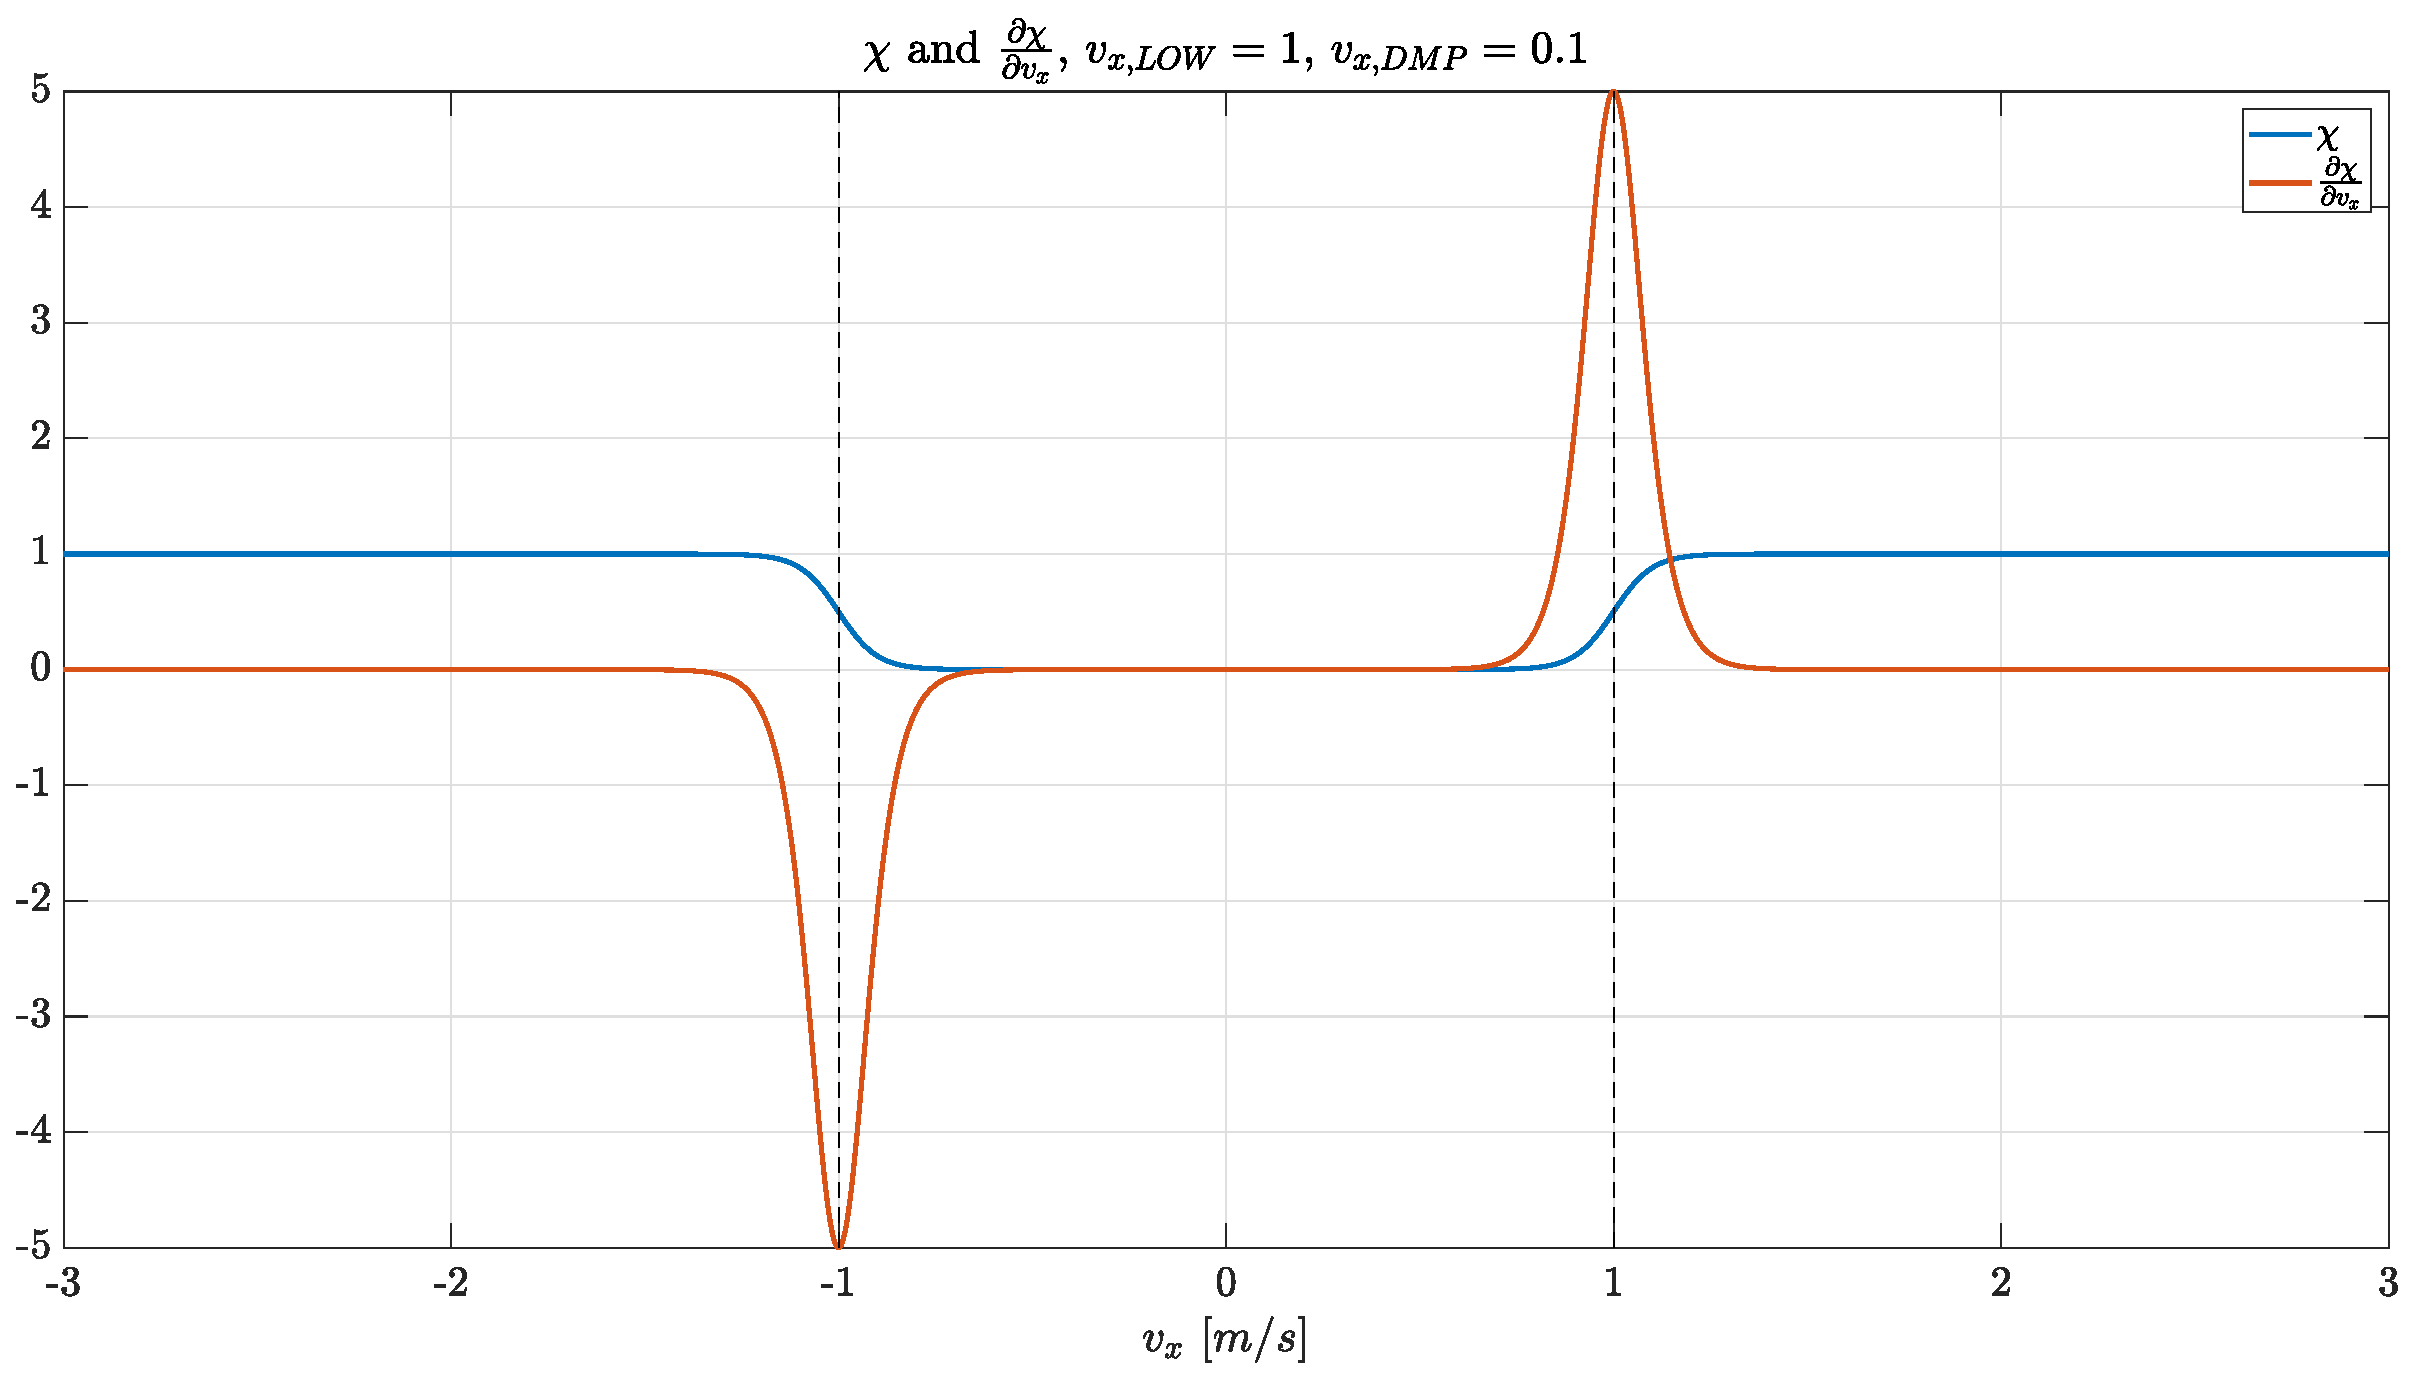
\includegraphics[width=1\textwidth]{MFTirePlots/transition.eps}
    \caption{$\chi$ and $\frac{\partial{\chi}}{\partial{v_x}}$}
\end{figure}
Finally, slip angle and slip ratio are expressed as:
\begin{equation}
    \begin{split}
        \alpha &= \chi \alpha_H + (1-\chi) \alpha_L\\
        \kappa &= \chi \kappa_H + (1-\chi) \kappa_L\\
    \end{split}
\end{equation}

\section{Tire forces}
At this point, the forces (which must be applied on the wheel hub) can be calculated:
\begin{equation}
    \begin{split}
        F_z &= k_t\left(r_0 + \rho\right)\\
        F_x &= F_z \mu_x(\kappa)\\
        F_y &= F_z \mu_y(\alpha)
    \end{split}
\end{equation}
Where
\begin{equation}
    \begin{split}
        \mu_x(\kappa) &= D_x\sin(C_x\arctan(B_x\kappa-E_x(B_x\kappa-\arctan(B_x\kappa))))\\
        \mu_y(\alpha) &= D_y\sin(C_y\arctan(B_y\alpha-E_y(B_y\alpha-\arctan(B_y\alpha))))\\
    \end{split}
\end{equation}
The total tire force can be obtained as:
\begin{equation}
    \mathbf{F} = F_z \mathbf{n} + F_x \mathbf{l} + F_y \mathbf{t}
\end{equation}
And finally, the transport moments
\begin{equation}
    \mathbf{M} = \rho\mathbf{r} \times \mathbf{F}
\end{equation}

\section{Jacobian Assembly}
Some of the most straightforward algebraic manipulations have been skipped in the documentation for brevity. Please refer to the $\textit{AssJac}$ function of the module for the full expressions for the partial jacobians.
\section{Vectors Perturbations}
\begin{equation}
    \begin{split}
        \Delta \mathbf{s} &= \boldsymbol{\theta}_{\Delta H} \times \mathbf{s}\\
        &= \left[\mathbf{s} \times ^T\right] \boldsymbol{\theta}_{\Delta H} \\
        &= \mathbf{J}_{\mathbf{s}} \boldsymbol{\theta}_{\Delta H}
    \end{split}
\end{equation}
\begin{equation}
    \begin{split}
        \Delta \mathbf{l} &= \left[\frac{\left(\mathbf{I}_{3\times3} - \mathbf{l} \otimes \mathbf{l}\right) \mathbf{n} \times}{||\mathbf{s} \times \mathbf{n}||} \mathbf{J}_{\mathbf{s}}\right] \boldsymbol{\theta}_{\Delta H} \\
        &= \mathbf{J}_{\mathbf{l}} \boldsymbol{\theta}_{\Delta H}
    \end{split}
\end{equation}
\begin{equation}
    \begin{split}
        \Delta \mathbf{t} &= \mathbf{n} \times \Delta \mathbf{l}\\
        &= \left[\mathbf{n} \times \mathbf{J}_\mathbf{l} \right]\boldsymbol{\theta}_{\Delta H}\\
        &= \mathbf{J}_\mathbf{t} \boldsymbol{\theta}_{\Delta H}
    \end{split}
\end{equation}
\begin{equation}
    \begin{split}
        \Delta \mathbf{r} &= \Delta \mathbf{l} \times \mathbf{s} + \mathbf{l} \times \Delta \mathbf{s}\\
        &= \left[{\mathbf{s} \times}^T \mathbf{J}_{\mathbf{l}} + {\mathbf{l} \times} \mathbf{J}_{\mathbf{s}}\right] \boldsymbol{\theta}_{\Delta H} \\
        &= \mathbf{J}_\mathbf{r} \boldsymbol{\theta}_{\Delta H}
    \end{split}
\end{equation}
\section{Vector derivatives perturbation}
\begin{equation}
    \begin{split}
        \Delta \dot{\mathbf{s}} &= \left[\boldsymbol{\omega}_R \times \mathbf{J}_s\right] \boldsymbol{\theta}_{\Delta H}  + \left[\mathbf{s} \times^T\right] \Delta \boldsymbol{\omega}_R \\
        &= \mathbf{J}_{{\dot{\mathbf{s}}}_{\boldsymbol{\theta}_{\Delta H}}} \boldsymbol{\theta}_{\Delta H} + \mathbf{J}_{{\dot{\mathbf{s}}}_{\boldsymbol{\omega}_R}} \Delta \boldsymbol{\omega}_R
    \end{split}
\end{equation}
\begin{equation}
    \begin{split}
        \Delta \dot{\mathbf{l}} = &\Bigg[
            \left(
                \left(\mathbf{l}^T \left(\mathbf{n} \times \dot{\mathbf{s}}\right)\right) \mathbf{I}_{3\times3}
                + \mathbf{l} \otimes \left(\mathbf{n} \times \dot{\mathbf{s}}\right)
            \right)
            \frac{\mathbf{J}_{\mathbf{l}}}{\|\mathbf{s} \times \mathbf{n}\|} \\
            &-
            \left(
                \left(\mathbf{I}_{3\times3} - \mathbf{l} \otimes \mathbf{l} \right)
                \left( \left( \mathbf{n} \times \dot{\mathbf{s}} \right) \otimes \mathbf{l} \right)
                \mathbf{n} \times
            \right)
            \frac{\mathbf{J}_{\mathbf{s}}}{\|\mathbf{s} \times \mathbf{n}\|^2} \\
            &-
            \left(
                \left( \mathbf{I}_{3\times3} - \mathbf{l} \otimes \mathbf{l} \right)
                \mathbf{n} \times
                \boldsymbol{\omega}_R \times
            \right)
            \frac{\mathbf{J}_{\mathbf{s}}}{\|\mathbf{s} \times \mathbf{n} \|}
        \Bigg] \boldsymbol{\theta}_{\Delta H} \\
        + &\left[\frac{\left(\mathbf{I}_{3\times3} - \mathbf{l} \otimes \mathbf{l} \right) \mathbf{n} \times \mathbf{s} \times}{\|\mathbf{s} \times \mathbf{n}\|}\right] \Delta \boldsymbol{\omega}_R\\
        &= \mathbf{J}_{{\dot{\mathbf{l}}}_{\boldsymbol{\theta}_{\Delta H}}}  \boldsymbol{\theta}_{\Delta H} + \mathbf{J}_{{\dot{\mathbf{l}}}_{\boldsymbol{\omega}_R}} \Delta \boldsymbol{\omega}_R
    \end{split}
\end{equation}
\begin{equation}
    \begin{split}
        \Delta \dot{\mathbf{r}} =
        &\left[
            \mathbf{s} \times^T \mathbf{J}_{\dot{\mathbf{l}}_{\boldsymbol{\theta}_{\Delta H}}}
            + \dot{\mathbf{l}} \times \mathbf{J}_{\mathbf{s}}
            + \dot{\mathbf{s}} \times^T \mathbf{J}_{\mathbf{l}}
            + \mathbf{l} \times \mathbf{J}_{\dot{\mathbf{s}}_{\boldsymbol{\theta}_{\Delta H}}}
        \right] \boldsymbol{\theta}_{\Delta H} \\
        + &\left[
            \mathbf{s} \times^T \mathbf{J}_{\dot{\mathbf{l}}_{\boldsymbol{\omega}_R}}
            + \mathbf{l} \times \mathbf{J}_{\dot{\mathbf{s}}_{\boldsymbol{\omega}_R}}
        \right] \Delta \boldsymbol{\omega}_R \\
        &= \mathbf{J}_{\dot{\mathbf{r}}_{\boldsymbol{\theta}_{\Delta H}}} \boldsymbol{\theta}_{\Delta H}
        + \mathbf{J}_{\dot{\mathbf{r}}_{\boldsymbol{\omega}_R}} \Delta \boldsymbol{\omega}_R
    \end{split}
\end{equation}
\section{Loaded radius perturbation}
\begin{equation}
    \begin{split}
        \Delta \rho &= -\frac{\rho}{\mathbf{r} \cdot \mathbf{n}} \mathbf{n}^T \mathbf{J}_{\mathbf{r}} \boldsymbol{\theta}_{\Delta H} - \frac{1}{\mathbf{r} \cdot \mathbf{n}} \mathbf{n}^T \Delta \dot{\mathbf{w}}_H \\
        &= \mathbf{J}_{\rho_{\boldsymbol{\theta}_{\Delta H}}} \boldsymbol{\theta}_{\Delta H} + \mathbf{J}_{\rho_{\dot{\mathbf{w}}_H}}\Delta \dot{\mathbf{w}}_H
    \end{split}
\end{equation}
\begin{equation}
    \begin{split}
        \Delta \dot{\rho} &= \left[-\frac{\mathbf{n}^T}{\mathbf{r} \cdot \mathbf{n}}\right] \Delta \dot{\mathbf{w}}_H \\
        &+ \left[-\frac{\mathbf{n}^T}{\mathbf{r} \cdot \mathbf{n}}\left(\dot{\mathbf{r}}\mathbf{J}_{\rho_{\boldsymbol{\theta}_{\Delta H}}} + \rho \mathbf{J}_{\dot{\mathbf{r}}_{\boldsymbol{\theta}_{\Delta H}}} + \dot{\rho}\mathbf{J}_{\mathbf{r}}\right)\right] \boldsymbol{\theta}_{\Delta H}\\
        &+ \left[-\frac{\mathbf{n}^T}{\mathbf{r} \cdot \mathbf{n}}\left(\dot{\mathbf{r}}\mathbf{J}_{\rho_{\mathbf{w}_H}}\right)\right] \Delta \mathbf{w}_H\\
        &+ \left[-\frac{\mathbf{n}^T}{\mathbf{r} \cdot \mathbf{n}}\left(\rho\mathbf{J}_{\dot{\mathbf{r}}_{\boldsymbol{\omega}_R}}\right)\right] \Delta \boldsymbol{\omega}_R \\
        &= \mathbf{J}_{\dot{\rho}_{\dot{\mathbf{w}}_H}}\Delta \dot{\mathbf{w}}_H + \mathbf{J}_{\dot{\rho}_{\boldsymbol{\theta}_{\Delta H}}} \boldsymbol{\theta}_{\Delta H} + \mathbf{J}_{\dot{\rho}_{\mathbf{w}_H}}\Delta \mathbf{w}_H + \mathbf{J}_{\dot{\rho}_{\boldsymbol{\omega}_R}} \Delta \boldsymbol{\omega}_R
    \end{split}
\end{equation}
\section{Velocities Perturbations}
\begin{equation}
    \begin{split}
        \Delta \mathbf{v}_{C} &= \Delta \dot{\mathbf{w}}_H + \Delta \dot{\rho} \mathbf{r} + \dot{\rho} \Delta \dot{\mathbf{r}} + \rho \Delta\dot{\mathbf{r}} \\
        &= \dots \\
        &= \mathbf{J}_{{\mathbf{v}_{C}}_{\dot{\mathbf{w}}_H}}\Delta \dot{\mathbf{w}}_H + \mathbf{J}_{{\mathbf{v}_{C}}_{\boldsymbol{\theta}_{\Delta H}}} \boldsymbol{\theta}_{\Delta H} + \mathbf{J}_{{\mathbf{v}_{C}}_{\mathbf{w}_H}}\Delta \mathbf{w}_H + \mathbf{J}_{{\mathbf{v}_{C}}_{\boldsymbol{\omega}_R}} \Delta \boldsymbol{\omega}_R
    \end{split}
\end{equation}
\begin{equation}
    \begin{split}
        \Delta \mathbf{v}_{C}^* &= \Delta \dot{\mathbf{w}}_H + \Delta \left(\frac{r_e}{\rho}\dot{\rho}\mathbf{r}\right) - r_e\Delta\dot{\mathbf{r}} \\
        &= \Delta \dot{\mathbf{w}}_H - \frac{r_e \mathbf{r}}{\rho} \Delta\dot{\rho} - \frac{r_e \dot{\rho}}{\rho} \Delta\mathbf{r} + r_e \frac{\dot{\rho}\mathbf{r}}{\rho^2}\Delta\rho - r_e\Delta\mathbf{r} \\
        &= \dots \\
        &= \mathbf{J}_{{\mathbf{v}_{C}^*}_{\dot{\mathbf{w}}_H}}\Delta \dot{\mathbf{w}}_H + \mathbf{J}_{{\mathbf{v}_{C}^*}_{\boldsymbol{\theta}_{\Delta H}}} \boldsymbol{\theta}_{\Delta H} + \mathbf{J}_{{\mathbf{v}_{C}^*}_{\mathbf{w}_H}}\Delta \mathbf{w}_H + \mathbf{J}_{{\mathbf{v}_{C}^*}_{\boldsymbol{\omega}_R}} \Delta \boldsymbol{\omega}_R
    \end{split}
\end{equation}
\begin{equation}
    \begin{split}
        \Delta \mathbf{v}_{S} &= \Delta \dot{\mathbf{w}}_H - r_e\left(\Delta\boldsymbol{\omega}_R \times \mathbf{r} + \boldsymbol{r} \times \Delta\mathbf{r}\right) \\
        &= \Delta \dot{\mathbf{w}}_H - r_e \mathbf{r} \times^T \Delta \boldsymbol{\omega}_R - r_e \boldsymbol{\omega}_R \times \Delta\mathbf{r}\\
        &= \dots \\
        &= \mathbf{J}_{{\mathbf{v}_{S}}_{\dot{\mathbf{w}}_H}}\Delta \dot{\mathbf{w}}_H + \mathbf{J}_{{\mathbf{v}_{S}}_{\boldsymbol{\theta}_{\Delta H}}} \boldsymbol{\theta}_{\Delta H} + \mathbf{J}_{{\mathbf{v}_{S}}_{\mathbf{w}_H}}\Delta \mathbf{w}_H + \mathbf{J}_{{\mathbf{v}_{S}}_{\boldsymbol{\omega}_R}} \Delta \boldsymbol{\omega}_R
    \end{split}
\end{equation}
\begin{equation}
    \begin{split}
        \Delta v_x &= \mathbf{l}^T \Delta\mathbf{v}_{C}^* + \mathbf{v}_{C}^*\Delta\mathbf{l}\\
        &= \dots \\
        &= \mathbf{J}_{{v_x}_{\dot{\mathbf{w}}_H}}\Delta \dot{\mathbf{w}}_H + \mathbf{J}_{{v_x}_{\boldsymbol{\theta}_{\Delta H}}} \boldsymbol{\theta}_{\Delta H} + \mathbf{J}_{{v_x}_{\mathbf{w}_H}}\Delta \mathbf{w}_H + \mathbf{J}_{{v_x}_{\boldsymbol{\omega}_R}} \Delta \boldsymbol{\omega}_R
    \end{split}
\end{equation}
\begin{equation}
    \begin{split}
        \Delta v_y &= \mathbf{t}^T \Delta\mathbf{v}_{C} + \mathbf{v}_{C}\Delta\mathbf{t}\\
        &= \dots \\
        &= \mathbf{J}_{{v_y}_{\dot{\mathbf{w}}_H}}\Delta \dot{\mathbf{w}}_H + \mathbf{J}_{{v_y}_{\boldsymbol{\theta}_{\Delta H}}} \boldsymbol{\theta}_{\Delta H} + \mathbf{J}_{{v_y}_{\mathbf{w}_H}}\Delta \mathbf{w}_H + \mathbf{J}_{{v_y}_{\boldsymbol{\omega}_R}} \Delta \boldsymbol{\omega}_R
    \end{split}
\end{equation}
\begin{equation}
    \begin{split}
        \Delta v_s &= \mathbf{l}^T \Delta\mathbf{v}_{S} + \mathbf{v}_{S}\Delta\mathbf{l}\\
        &= \dots \\
        &= \mathbf{J}_{{v_s}_{\dot{\mathbf{w}}_H}}\Delta \dot{\mathbf{w}}_H + \mathbf{J}_{{v_s}_{\boldsymbol{\theta}_{\Delta H}}} \boldsymbol{\theta}_{\Delta H} + \mathbf{J}_{{v_s}_{\mathbf{w}_H}}\Delta \mathbf{w}_H + \mathbf{J}_{{v_s}_{\boldsymbol{\omega}_R}} \Delta \boldsymbol{\omega}_R
    \end{split}
\end{equation}
\section{Slip Quantities Perturbations}
\begin{equation}
    \begin{split}
        \Delta \alpha_H &= \left[\frac{v_x}{v_x^2 + v_y^2} \mathbf{J}_{{v_y}_{\boldsymbol{\theta}_{\Delta H}}} - \frac{v_y}{v_x^2 + v_y^2}\mathbf{J}_{{v_x}_{\boldsymbol{\theta}_{\Delta H}}}\right] \boldsymbol{\theta}_{\Delta H}\\
        &+ \left[\frac{v_x}{v_x^2 + v_y^2} \mathbf{J}_{{v_y}_{\dot{\mathbf{w}}_H}} - \frac{v_y}{v_x^2 + v_y^2}\mathbf{J}_{{v_x}_{\dot{\mathbf{w}}_H}}\right] \Delta {\dot{\mathbf{w}}}_H\\
        &+ \left[\frac{v_x}{v_x^2 + v_y^2} \mathbf{J}_{{v_y}_{\boldsymbol{\omega}_R}} - \frac{v_y}{v_x^2 + v_y^2}\mathbf{J}_{{v_x}_{\boldsymbol{\omega}_R}}\right] \Delta \boldsymbol{\omega}_R\\
        &- \left[\frac{v_y}{v_x^2 + v_y^2}\mathbf{J}_{{v_x}_{{\mathbf{w}}_H}}\right] \Delta {\mathbf{w}}_H\\
        &= \mathbf{J}_{{\alpha_H}_{\boldsymbol{\theta}_{\Delta H}}}\boldsymbol{\theta}_{\Delta H} + \mathbf{J}_{{\alpha_H}_{\dot{\mathbf{w}}_H}}\Delta {\dot{\mathbf{w}}}_H + \mathbf{J}_{{\alpha_H}_{\boldsymbol{\omega}_R}}\Delta \boldsymbol{\omega}_R + \mathbf{J}_{{\alpha_H}_{\mathbf{w}_H}}\Delta {\mathbf{w}}_H\\
        \Delta \kappa_H &= \frac{\Delta v_s}{v_x} - \frac{v_s}{v_x^2}\Delta v_x\\
        &= \dots \\
        &= \mathbf{J}_{{\kappa_H}_{\boldsymbol{\theta}_{\Delta H}}}\boldsymbol{\theta}_{\Delta H} + \mathbf{J}_{{\kappa_H}_{\boldsymbol{\omega}_R}}\Delta \boldsymbol{\omega}_R + \mathbf{J}_{{\kappa_H}_{\dot{\mathbf{w}}_H}}\Delta {\dot{\mathbf{w}}}_H + \mathbf{J}_{{\kappa_H}_{\mathbf{w}_H}}\Delta {\mathbf{w}}_H
    \end{split}
\end{equation}
\begin{equation}
    \begin{split}
        \Delta \alpha_L &= \Delta v_y\\
        \Delta \kappa_L &= \Delta v_s\\
    \end{split}
\end{equation}
\begin{equation}
    \begin{split}
        \Delta \kappa &= \frac{\partial\kappa}{\partial\chi}\Delta\chi + \frac{\partial\kappa}{\partial\kappa_L}\Delta\kappa_L + \frac{\partial\kappa}{\partial\kappa_H}\Delta\kappa_H \\
        &= \cdots \\
        &= \mathbf{J}_{\kappa_{\boldsymbol{\theta}_{\Delta H}}}\boldsymbol{\theta}_{\Delta H} + \mathbf{J}_{\kappa_{\boldsymbol{\omega}_R}}\Delta \boldsymbol{\omega}_R + \mathbf{J}_{\kappa_{\dot{\mathbf{w}}_H}}\Delta {\dot{\mathbf{w}}}_H + \mathbf{J}_{\kappa_{\mathbf{w}_H}}\Delta {\mathbf{w}}_H
    \end{split}
\end{equation}
\begin{equation}
    \begin{split}
        \Delta \alpha &= \frac{\partial\alpha}{\partial\chi}\Delta\chi + \frac{\partial\alpha}{\partial\alpha_L}\Delta\alpha_L + \frac{\partial\alpha}{\partial\alpha_H}\Delta\alpha_H \\
        &= \cdots \\
        &= \mathbf{J}_{\alpha_{\boldsymbol{\theta}_{\Delta H}}}\boldsymbol{\theta}_{\Delta H} + \mathbf{J}_{\alpha_{\dot{\mathbf{w}}_H}}\Delta {\dot{\mathbf{w}}}_H + \mathbf{J}_{\alpha_{\boldsymbol{\omega}_R}}\Delta \boldsymbol{\omega}_R + \mathbf{J}_{\alpha_{\mathbf{w}_H}}\Delta {\mathbf{w}}_H\\
    \end{split}
\end{equation}

\section{Tire Forces and Moments Perturbation}
\begin{equation}
    \begin{split}
        \Delta F_z &= k_t \Delta \rho\\
        &= \cdots \\
        &= \mathbf{J}_{{F_z}_{\boldsymbol{\theta}_{\Delta H}}}\boldsymbol{\theta}_{\Delta H} + \mathbf{J}_{{F_z}_{\mathbf{w}_H}}\Delta \mathbf{w}_H\\
        \Delta F_x &= \Delta F_z \mu_x(\kappa) + F_z \Delta \mu_x(\kappa)\\
        &= \cdots \\
        &= \mathbf{J}_{{F_x}_{\boldsymbol{\theta}_{\Delta H}}}\boldsymbol{\theta}_{\Delta H} + \mathbf{J}_{{F_x}_{\mathbf{w}_H}}\Delta \mathbf{w}_H + \mathbf{J}_{{F_x}_{\dot{\mathbf{w}}_H}}\Delta {\dot{\mathbf{w}}}_H + \mathbf{J}_{{F_x}_{\boldsymbol{\omega}_R}}\Delta \boldsymbol{\omega}_R\\
        \Delta F_y &= \Delta F_z \mu_y(\alpha) + F_z \Delta \mu_y(\alpha)\\
        &= \cdots \\
        &= \mathbf{J}_{{F_y}_{\boldsymbol{\theta}_{\Delta H}}}\boldsymbol{\theta}_{\Delta H} + \mathbf{J}_{{F_y}_{\mathbf{w}_H}}\Delta \mathbf{w}_H + \mathbf{J}_{{F_y}_{\dot{\mathbf{w}}_H}}\Delta {\dot{\mathbf{w}}}_H + \mathbf{J}_{{F_y}_{\boldsymbol{\omega}_R}}\Delta \boldsymbol{\omega}_R\\
    \end{split}
\end{equation}
\begin{equation}
    \begin{split}
        \Delta \mathbf{F} &= \Delta F_z \mathbf{n} + \Delta F_x \mathbf{l} + F_x \Delta \mathbf{l} + \Delta F_y \mathbf{t} + F_y \Delta \mathbf{t}\\
        &= \cdots \\
        &= \mathbf{J}_{\mathbf{F}_{\boldsymbol{\theta}_{\Delta H}}}\boldsymbol{\theta}_{\Delta H} + \mathbf{J}_{\mathbf{F}_{\mathbf{w}_H}}\Delta \mathbf{w}_H + \mathbf{J}_{\mathbf{F}_{\dot{\mathbf{w}}_H}}\Delta {\dot{\mathbf{w}}}_H + \mathbf{J}_{\mathbf{F}_{\boldsymbol{\omega}_R}}\Delta \boldsymbol{\omega}_R\\
    \end{split}
\end{equation}
\begin{equation}
    \begin{split}
        \Delta \mathbf{M} &= \Delta(\rho\mathbf{r}) \times \mathbf{F} + \rho\mathbf{r} \times \Delta\mathbf{F}\\
        &= \Delta\rho \mathbf{r} \times \mathbf{F} + \rho \Delta\mathbf{r} \times \mathbf{F} + \rho\mathbf{r} \times \Delta\mathbf{F}\\
        &= \cdots \\
        &= \mathbf{J}_{\mathbf{M}_{\boldsymbol{\theta}_{\Delta H}}}\boldsymbol{\theta}_{\Delta H} + \mathbf{J}_{\mathbf{M}_{\mathbf{w}_H}}\Delta \mathbf{w}_H + \mathbf{J}_{\mathbf{M}_{\dot{\mathbf{w}}_H}}\Delta {\dot{\mathbf{w}}}_H + \mathbf{J}_{\mathbf{M}_{\boldsymbol{\omega}_R}}\Delta \boldsymbol{\omega}_R\\
    \end{split}
\end{equation}

\section{Updated-updated approximation}

The Jacobian matrix is the following:
\begin{equation}
    \begin{bmatrix}
        \Delta \mathbf{F} \\ \Delta \mathbf{M}
    \end{bmatrix} = \begin{bmatrix}
        \mathbf{J}_{\mathbf{F}_{\mathbf{w}_H}} && \mathbf{J}_{\mathbf{F}_{\dot{\mathbf{w}}_H}} && \mathbf{J}_{\mathbf{F}_{\boldsymbol{\theta}_{\Delta H}}} &&  \mathbf{J}_{\mathbf{F}_{\boldsymbol{\omega}_R}}\\
        \mathbf{J}_{\mathbf{M}_{\mathbf{w}_H}} && \mathbf{J}_{\mathbf{M}_{\dot{\mathbf{w}}_H}} && \mathbf{J}_{\mathbf{M}_{\boldsymbol{\theta}_{\Delta H}}} && \mathbf{J}_{\mathbf{M}_{\boldsymbol{\omega}_R}}
    \end{bmatrix}\begin{bmatrix}
        \Delta \mathbf{w}_H \\ \Delta {\dot{\mathbf{w}}}_H \\ \boldsymbol{\theta}_{\Delta H} \\ \Delta \boldsymbol{\omega}_R
    \end{bmatrix}
\end{equation}
The following approximations are introduced:
\begin{equation}
    \begin{split}
        \Delta \mathbf{w} &= \text{dCoef} \Delta {\dot{\mathbf{w}}}\\
        \boldsymbol{\theta}_{\Delta} &= \text{dCoef} \Delta {\dot{\mathbf{g}}}\\
        \Delta \boldsymbol{\omega} &= \left(\mathbf{I}_{3\times3} - \text{dCoef}\boldsymbol{\omega}\times\right)\Delta {\dot{\mathbf{g}}}
    \end{split}
\end{equation}
Finally,
\begin{equation}
    \begin{bmatrix}
        \Delta \mathbf{F} \\ \Delta \mathbf{M}
    \end{bmatrix} = \begin{bmatrix}
        \mathbf{J}_{\mathbf{F}_{\mathbf{w}_H}} + \text{dCoef}\mathbf{J}_{\mathbf{F}_{\dot{\mathbf{w}}_H}} && \text{dCoef}\mathbf{J}_{\mathbf{F}_{\boldsymbol{\theta}_{\Delta H}}} && \mathbf{J}_{\mathbf{F}_{\boldsymbol{\omega}_R}}\left(\mathbf{I}_{3\times3} - \text{dCoef}\boldsymbol{\omega}_R\times\right)\\
        \mathbf{J}_{\mathbf{M}_{\mathbf{w}_H}} + \text{dCoef}\mathbf{J}_{\mathbf{M}_{\dot{\mathbf{w}}_H}} && \text{dCoef}\mathbf{J}_{\mathbf{M}_{\boldsymbol{\theta}_{\Delta H}}} && \mathbf{J}_{\mathbf{M}_{\boldsymbol{\omega}_R}}\left(\mathbf{I}_{3\times3} - \text{dCoef}\boldsymbol{\omega}_R\times\right)\\
    \end{bmatrix}\begin{bmatrix}
        \Delta {\dot{\mathbf{w}}}_H  \\ \Delta \dot{\mathbf{g}}_H \\ \Delta \dot{\mathbf{g}}_R
    \end{bmatrix}
\end{equation}

\section{Addendum: $\chi$ and $\mu$ derivatives}
\label{ss:derivatives}

\begin{equation}
    \frac{\partial{\chi}}{\partial{v_x}} = \frac{v_x \cosh\left(\frac{|v_x| - v_{x,\text{LOW}}}{v_{x, \text{DMP}}}\right)^{-2}}{2v_{x, \text{DMP}}|v_x|}
\end{equation}

\begin{equation}
    \frac{\partial{\mu_x}}{\partial{\kappa}} = -C_xD_x\left(E_x\left(B_x - \frac{B_x}{B_x^2\kappa^2 + 1}\right) - B_x\right)\frac{\cos\left(C_x\arctan\left(E_x\left(B_x\kappa - \arctan(B_x\kappa)\right) - B_x\kappa\right)\right)}{(E_x(B_x\kappa - \arctan(B_x\kappa)) - B_x\kappa)^2 + 1}
\end{equation}

\begin{equation}
    \frac{\partial{\mu_y}}{\partial{\alpha}} = -C_yD_y\left(E_y\left(B_y - \frac{B_y}{B_y^2\alpha^2 + 1}\right) - B_y\right)\frac{\cos\left(C_y\arctan\left(E_y\left(B_y\alpha - \arctan(B_y\alpha)\right) - B_y\alpha\right)\right)}{(E_y(B_y\alpha - \arctan(B_y\alpha)) - B_y\alpha)^2 + 1}
\end{equation}

\section{Jacobian Validation}
Given the amount of calculations involved in the Jacobian matrix assembly, a validation process has been carried out to ensure the correctness of the resulting terms.

Two MATLAB functions have been written to accomplish the task.

$\textit{TestJac}$ implements the formulas to verify their validity by checking that the Jacobian terms effectively appoximate the nonlinear functions over small increments of each degree of freedom. Figure~\ref{fig:jac} shows how the comparison is carried out.

\begin{figure}
    \label{fig:jac}
    \centering
    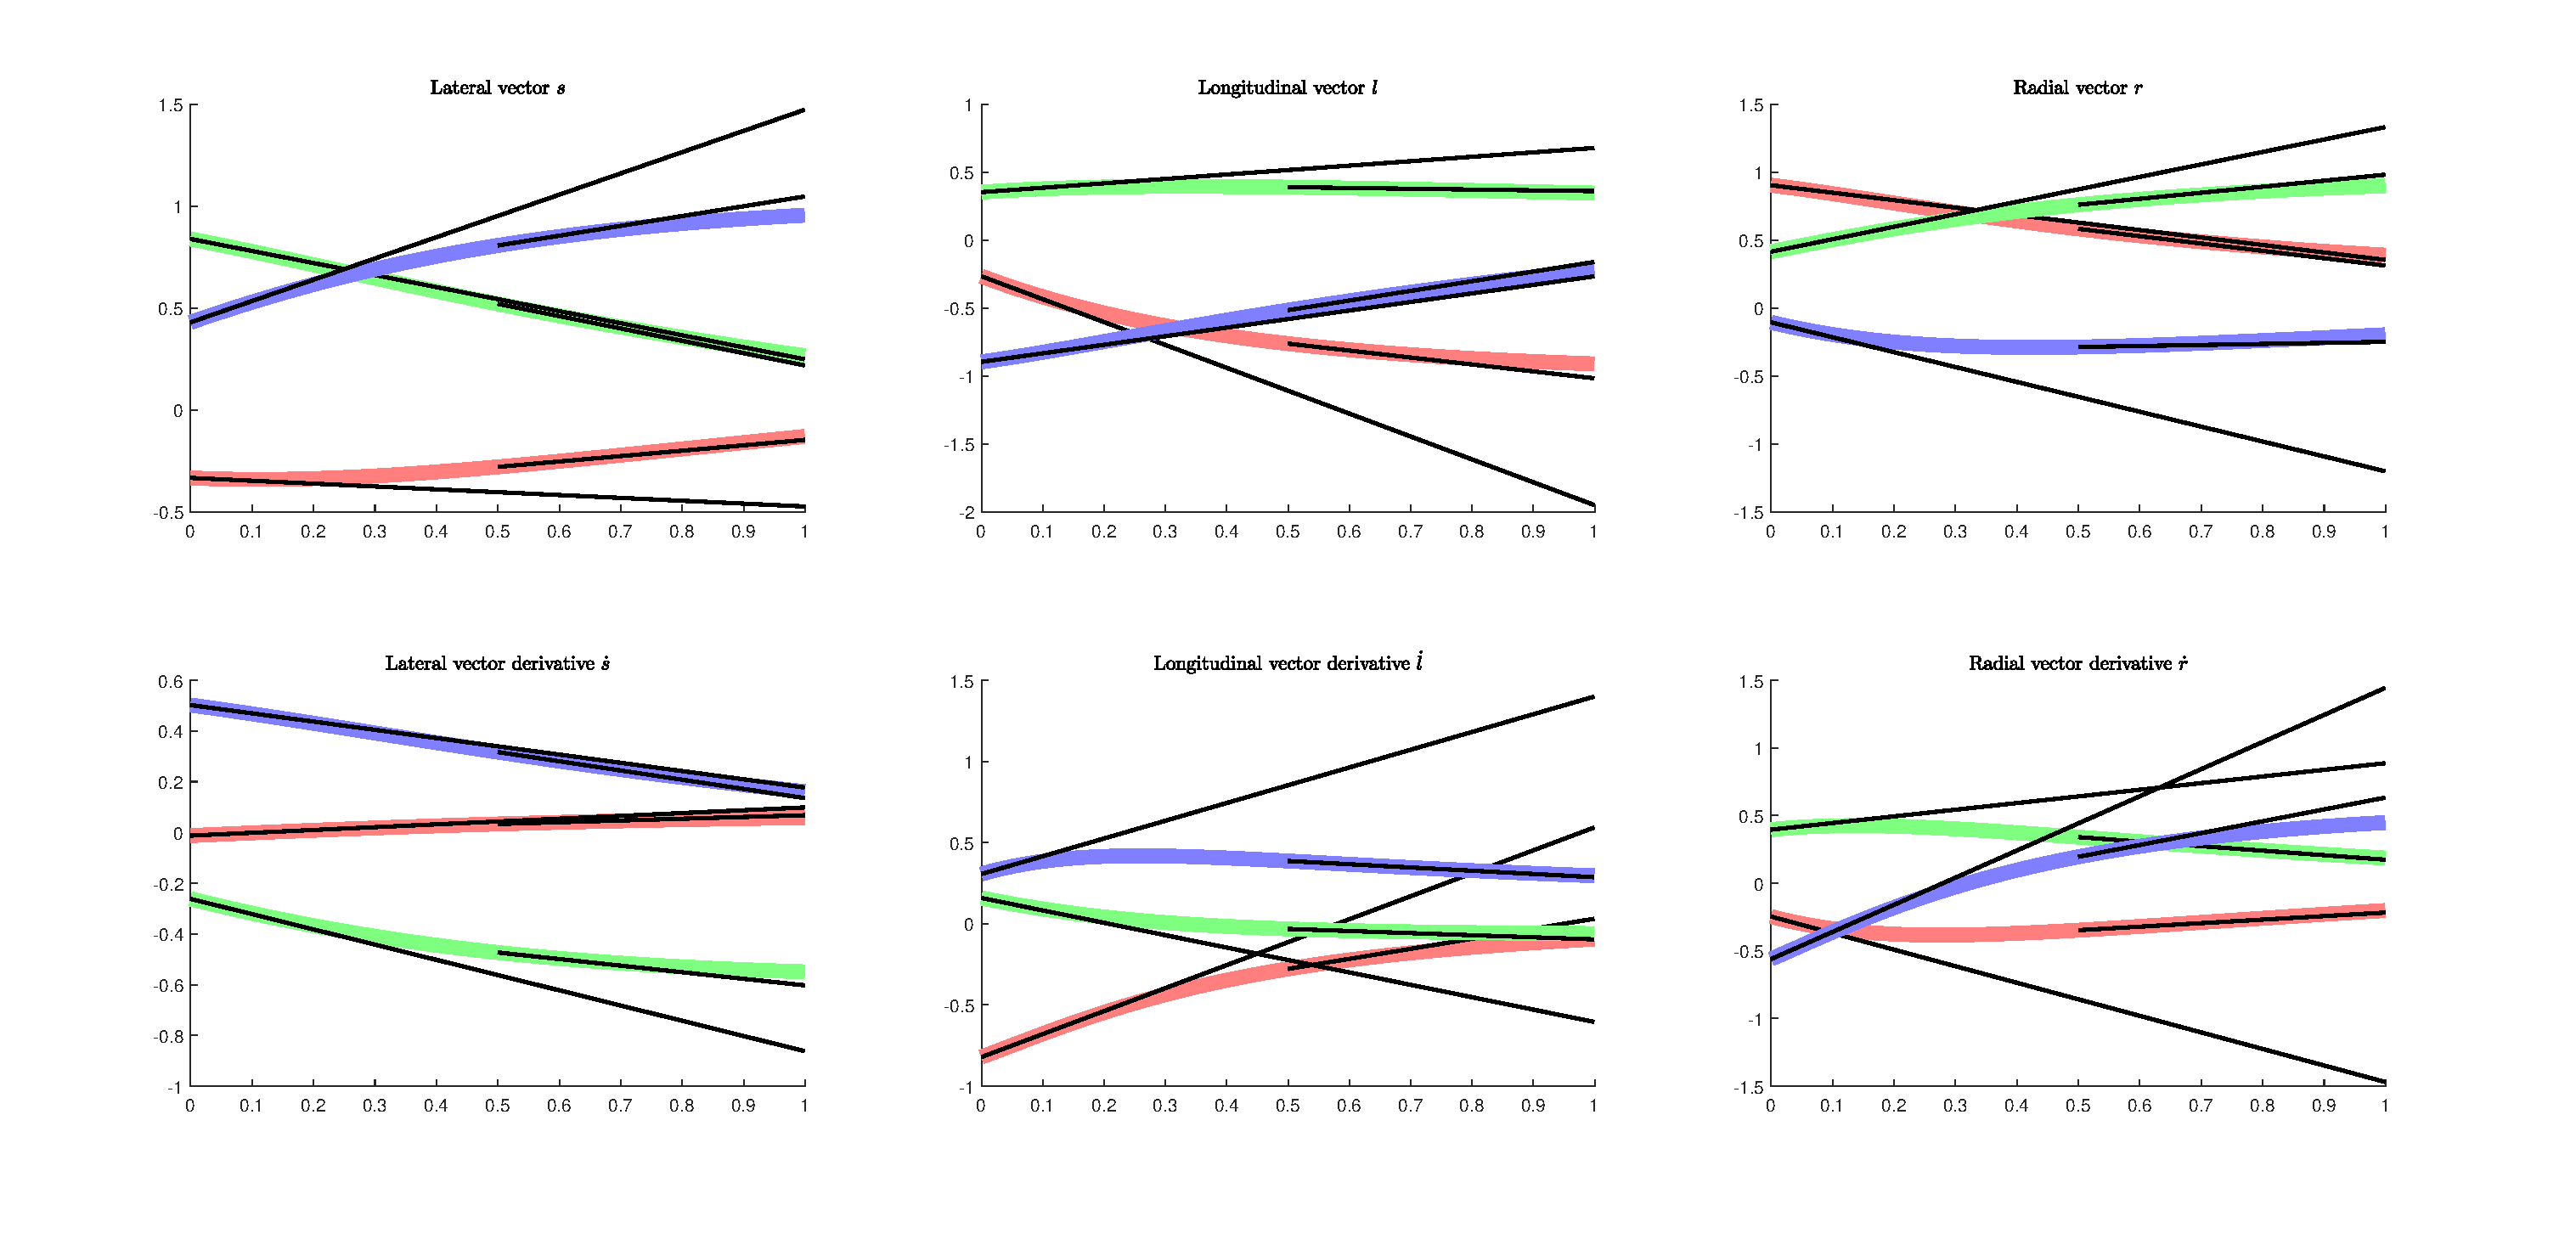
\includegraphics[width=1\textwidth]{MFTirePlots/jac.eps}
    \caption{Validation of each component of the unit vectors}
\end{figure}

$\textit{ValidJac}$ is meant to check that the implementation of the formulas in the module yields the correct numeric values of the jacobian terms. A few timesteps are simulated in MBDyn, the values of the degrees of freedom are passed to the function which returns the jacobian components, which are directly compared with the ones calculated by the module.
